\documentclass[11pt,dvipsnames]{report} % {{{
\usepackage[spanish]{babel}
\usepackage[utf8]{inputenc}
\usepackage[T1]{fontenc}
\usepackage{makeidx}
\usepackage{graphicx}
\usepackage{subfig}
\usepackage{amsmath}
\usepackage{amsfonts}
\usepackage{amssymb}
\usepackage{authblk} % para la manipulación de autores y afiliación
\usepackage[pdftex]{hyperref}
\usepackage{multirow}
\usepackage{multicol}
\usepackage{float}
\usepackage{xcolor}
\usepackage{booktabs}
\usepackage{colortbl}
\usepackage{bbold}
\usepackage{physics}
\usepackage{mathtools}
\usepackage{dsfont}
\usepackage{tensor}

% Theorems, proofs, etc
\usepackage{amsthm}



\usepackage{fancybox}
\usepackage{colortbl}
\usepackage{amsbsy}
\usepackage[draft,inline,nomargin]{fixme} \fxsetup{theme=color}

%This defines my comments
\definecolor{mycolor}{RGB}{255,50,0}
\FXRegisterAuthor{ja}{aja}{\color{mycolor}JA}


\usepackage[]{lineno} \linenumbers
\setlength\linenumbersep{3pt}

\newcommand{\fref}[1]{fig.~\ref{#1}}  \newcommand{\tref}[1]{table~\ref{#1}}
\newcommand{\Fref}[1]{Fig.~\ref{#1}}  \newcommand{\Tref}[1]{Table~\ref{#1}}

\usepackage{hyperref}
%\usepackage{commath}
\decimalpoint
\renewcommand{\tablename}{Tabla}
\oddsidemargin 0in
\textwidth 6.5in
\topmargin -0.5in
\textheight 8.5in

\newcommand{\psii}{\psi_i}
\newcommand{\Pk}[1]{\ket{\psi_{#1} }}
\newcommand{\Pb}[1]{\bra{\psi_{#1} }}
\newcommand{\pk}{\ket{\psi}}
\newcommand{\M}{\mathcal{M}^{(N)}}
\newcommand{\E}{\mathcal{E}}
\newcommand{\Erho}{\mathcal{E}(\rho)}
\newcommand{\1}{\mathds{1}}
\newcommand{\ten}{\otimes}
\newcommand{\h}[1]{\colorbox{Yellow}{#1}}
\newcommand{\hi}{\mathcal{H}}
\newcommand{\txt}[1]{\text{#1}}
\newcommand{\here}{\h{\hspace{15cm}} }
\newcommand{\rhoi}{\dyad{\psii}{\psii}}
\newcommand{\ind}[2]{{{}^{#1}_{#2}}}
\newcommand{\QH}{\abs{Q_H}}
\newcommand{\QL}{\abs{Q_L}}
\newcommand{\W}{\abs{W}}

\def\dbar{{\mathchar'26\mkern-12mu d}}


% Para que funcione mejor la numeración {{{
% https://tex.stackexchange.com/questions/43648/why-doesnt-lineno-number-a-paragraph-when-it-is-followed-by-an-align-equation
\newcommand*\patchAmsMathEnvironmentForLineno[1]{%
  \expandafter\let\csname old#1\expandafter\endcsname\csname #1\endcsname
  \expandafter\let\csname oldend#1\expandafter\endcsname\csname end#1\endcsname
  \renewenvironment{#1}%
     {\linenomath\csname old#1\endcsname}%
     {\csname oldend#1\endcsname\endlinenomath}}% 
\newcommand*\patchBothAmsMathEnvironmentsForLineno[1]{%
  \patchAmsMathEnvironmentForLineno{#1}%
  \patchAmsMathEnvironmentForLineno{#1*}}%
\AtBeginDocument{%
\patchBothAmsMathEnvironmentsForLineno{equation}%
\patchBothAmsMathEnvironmentsForLineno{align}%
\patchBothAmsMathEnvironmentsForLineno{flalign}%
\patchBothAmsMathEnvironmentsForLineno{alignat}%
\patchBothAmsMathEnvironmentsForLineno{gather}%
\patchBothAmsMathEnvironmentsForLineno{multline}%
}
% }}}
% }}}
\title{Notas de estudio para Examen Privado\\
Licenciatura en Física}
\author{J.A. de León}

\newtheorem{definition}{Definición}[section]

\newtheorem{teorema}{Teorema}[section]

\newtheorem{property}{Propiedad}[section]

\begin{document}
\maketitle

\chapter{Termodinámica}
\section{Trabajo}
\begin{enumerate}
\item Durante un \textbf{proceso cuasiestático} un sistema atraviesa 
		en todo momento 
	  estados infinitesimalmente cercanos al equilibrio termodinámico y, 
	  por consiguiente, la dinámica de los estados puede ser descrita
	  en términos de coordenadas termodinámicas $\Rightarrow$ existe 
	  una ecuación de estado que describe estos estados 
\item Equilibrio termodinámico: eq. mecánico $+$ eq. térmico $+$ 
 	  eq. químico
\item Diferencial de trabajo de un sistema de un gas en un pistón:
\begin{equation}
\dbar W= PAdx = -PdV,
\end{equation}
el signo negativo asegura que en una compresión $(dV<0)$ $\dbar W>0$ 
(trabajo sobre el sistema, i.e. el sistema gana energía). 
\item El trabajo realizado sobre un sistema hidrostático depende de 
la trayectoria que se siga en el diagrama de estados (a diferencia
del trabajo realizado por la fuerza gravitacional, por ej). 
\item El trabajo relizado sobre un gas, definido por
\begin{align*}
W=-\int_{V_i}^{V_f} PdV, 
\end{align*}
se puede integrar siempre y cuando se conozca una función 
de estado.
\item ¡¡¡Calor $=$ energía!!!
\end{enumerate}

\section{1era ley de la Termodinámica}
\begin{itemize}
\item Una forma \textbf{restringida} de enunciar la primera ley 
de la termodinámica es:

Si un sistema cerrado es causado a cambiar de estado de un estado 
inicial a un estado final únicamente por procesos adiabáticos, entonces
el trabajo realizado sobre el sistema es el mismo para todas las trayectorias
adiabáticas que conectan a ambos estados. 

Es restringida porque no se está diciendo qué ocurre en 
aquellos procesos no adiabáticos. Es decir, en procesos
en los que ocurre intercambio de calor. 
\item Se sigue de esta forma restringida de la primera ley de la 
Termodinámica que existe una función que depende únicamente
de las coordenadas termodinámicas cuya diferencia entre el valor
final e inicial es igual al trabajo adiabático que se realiza al
sistema pasar del estado inicial al estado final. Esta función 
es la función de \textbf{energía interna} $U$: 
\begin{align}
W_{i\to f}\text{(adiabático)}=U_f-U_i,
\end{align}
esta diferencia da el aumento en energía interna del sistema. 
\item  \textbf{1era. ley de la Termodinámica} (formulación 
matemática): 
Cuando un sistema cerrado y su entorno se encuentran a distintas
temperatura y se realiza trabajo diatérmico [?] sobre el sistema,
entonces la energía transferida por otros procesos no mecánicos, 
igual a la diferencia entre el cambio de energía interna y el 
trabajo diatérmano se llama calor $Q$:
\begin{align}
  \Delta U = Q + W,
  \label{eq:1st-law-thermodynamics}
\end{align}
donde $Q>0$ cuando el calor entra al sistema y $Q<0$ cundo
abandona el sistema. Tres ideas están plasmadas en 
\eqref{eq:1st-law-thermodynamics}: (1) la existencia de una 
función de energía interna, (2) el principio de conservación de 
la energía, y (3) la definición de trabajo como energía en tránsito
en virtud de una diferencia de temperatura.
\item \textbf{Forma diferencial de la 1era. ley de la Termodinámica}:
para un sistema termodinámico que atraviesa cambios infinitesimales 
en sus variables termodinámicas la primera ley se formula como
\begin{align}
  dU = \dbar Q + \dbar W.
  \label{eq:1st-law-thermodynamics_diffForm}
\end{align}
\item \textbf{Capacidad calorífica}: 
\begin{align}
  C=\dv{Q}{T} \qty[\frac{K}{J}]
  \label{eq:heat-capacity}.
\end{align}
\item El caso de un gas:

La ecuación \eqref{eq:1st-law-thermodynamics_diffForm} toma 
la forma 
\begin{align}
   dU =\dbar Q-PdV,
   \label{eq:1st-law-gas}
 \end{align} 
donde $U$ es una función de algún par $P,V,T$ (la ecuación relaciona 
a un par con la tercera). Tomando $U=U(T,V)$ se tiene 
\begin{align*}
dU=\qty(\pdv{U}{T	})_VdT+\qty(\pdv{U}{V})_TdV,
\end{align*}
y sustityendo en \eqref{eq:1st-law-gas}
\begin{align*}
\dbar Q &=\qty(\pdv{U}{T	})_VdT+\qty[\qty(\pdv{U}{V})_T+P]dV\\
\dv{Q}{T} &= \qty(\pdv{U}{T	})_V
+\qty[\qty(\pdv{U}{V})_T+P]\dv{V}{T}.
\end{align*}
\item Flujo cuasiestático de calor: cuando a lo largo de un sistema 
existe un gradiente de temperatura y el calor fluye de manera
cuasiestática (misma definición) podemos calcular el 
calor que se absorbe durante el proceso utilizando la ecuación 
\eqref{eq:heat-capacity} de la capacidad calorífica.
\item El transporte de energía en un sistema entre elementos
de volumen vecinos en virtud de una diferencia de temperatura se 
conoce como conducción de calor. Los experimentos muestran que 
\begin{align*}
\frac{Q}{t}\propto A\frac{\Delta T}{\Delta x},
\end{align*}
con $A$ el área transversal al flujo de calor. Por consiguiente
\begin{align}
\dv{Q}{t	} = -KA\dv{T}{x},
\end{align}
con $K$ la conductividad térmica. El signo menos es para asegurar
que la dirección del flujo de calor sea en la dirección positiva de $x$.
\item \textbf{Radiación térmica}: radiación en virtud de su temperatura.
\item Exitancia radiante $\mathcal{R}$: potencia irradiada total por 
unidad de área. Emisividad total $\epsilon$: fracción de la potencia
irradiada total que es emitida como radiación térmica.
\item \textbf{Ley de Stefan-Boltzmann}: un cuerpo negro es una
sustancia ideal que es capaz de absorber toda la luz incidente 
sobre ella y reemitirla netamente como radiación térmica. La
radiación de un cuerpo como este está dada por la la siguiente ley:
\begin{align}
  \mathcal{R}=\mathcal{R}(T)=\sigma T^4,
  \label{eq:stefan-boltzmann}
\end{align}
donde $\sigma$ es la constante de Stefan-Boltzmann.
\end{itemize}

\section{Gas ideal}
\begin{enumerate}
\item \textbf{Expansión libre adiabática}: gas en expansión en el 
cual no se hace trabajo ni se transfiere calor $\Rightarrow$ $\Delta U=0$
durante la expansión libre.
\item Al escribir explícitamente $dU$ asumiendo que $U=U(T,V)$ ó 
$U=U(T,P)$ y al considerar una expansión libre adiabática $(dU=0)$
se concluye que $U=U(T)$ para un gas ideal. 
\item Un \textbf{gas ideal} satisface
\begin{align}
  PV&=nRT, & \qty(\pdv{U}{P})_T&=0,
  \label{eq:ideal-gas}
\end{align}
la primera condición es la ecuación de estado del gas ideal y 
la segunda es para asegurar que en una expansión libre
$dU=0$.
\item Retomando la ecuación \eqref{eq:1st-law-gas}:
\begin{align*}
\dbar Q=dU+PdV,
\end{align*}
cuando $dV=0$
\begin{align*}
\qty(\dv{Q}{T})_T=C_V=\qty(\pdv{U}{T})_V.
\end{align*}
En el caso del gas ideal $U=U(T)$, por consiguiente
\begin{align*}
C_V=\dv{U}{T},
\end{align*}
y 
\begin{align*}
\dbar Q = C_VdT+PdV,
\end{align*}
y sacando un diferencial de la ecuación de estado del gas ideal
\begin{align*}
PdV+VdP=nRdT.
\end{align*}
Sustiyendo arriba
\begin{align*}
\dbar Q &= C_VdT + nRdT - VdP\\
\dv{Q}{T}&=\qty(C_V+nR)-V\dv{P}{T},
\end{align*}
cuando $dP=0$:
\begin{align}
  \qty(\dv{Q}{T})_P=C_P=C_V+nR.
  \label{eq:C_P-idealGas}
\end{align}
\end{enumerate}




































\chapter{Mecánica Estadística}


\section{Fundamentos estadísticos de la Termodinámica}
\begin{itemize}
	\item La especificación de los valores de los parámetros $N$, $V$ y $E$
	define a un \textbf{macroestado}.
	
	\item Los \textbf{microestados} se identifican como las posibles 
	configuraciones de un sistema para dar lugar al mismo valor 
	de energía $E$ del sistema completo, $\Omega=\Omega(N,V,E).$
	
	\item \textbf{Postulado de la igualdad de probabilidad apriori:} el sistema
	tiene igualdad de probabilidad de estar en cualquiera de los posibles
	microestados.
	
	\item Al colocar dos sistemas termodinámicos en contacto se supone
	que estos llegarán al equilibrio cuando se el valor de la energía
	del sistema (\janote{del sistema?}) maximice el número 
	de microestados en los que se puede encontrar el sistema.
	El macroestado con la mayor cantidad de microestados 
	se dice que es el más probable.
	
	\item $S=k\ln \Omega$: entropía absoluta en términos del número
	total de microestados accesibles según el macroestado del sistema.
	
	\item De la fórmula que enunció Planck sobre la entropía (ya había
	sido formulada por Boltzmann, pero fue Planck quien la escribió en la
	forma moderna) se desprende que la entropía se hace cero cuando 
	el sistema puede encontrarse en una sola configuración.
	
	\item \textbf{El gas ideal clásico}: dado que asumimos que las 
	partículas no interactúan entre sí dentro del gas, entonces
	\begin{align}
	\Omega (N,E,V)\propto V^N,
	\end{align}
	y esto nos lleva a que 
	\begin{align}
	\pdv{S}{V}&=\frac{P}{T}=k\qty(\pdv{\ln \Omega \qty(N,E,V)}{V})_{N,E}=
	k\frac{N}{V}  \\
	PV&=kNT = nRT \hspace{1.5cm} (R=kN_A),
	\end{align}
	así hemos llegado a la ecuación de estado del gas ideal desde 
	principios estadísticos.
	
	\item \textbf{Paradoja de Gibbs (entropía de mezcla):} Gibbs consideró
	una situación como la de la \Fref{fig:gibbs-paradox} en la que 2 gases
	iguales se mantienen a ambos lados de una pared diatérmana, luego
	la pared se quita y se permite que ambos gases se mezclen. En este 
	caso particular tenemos un proceso reversible porque podemos 
	volver a colocar la pared y tendríamos la misma situación inicial. 
	Sin embargo, con métodos estadísticos se concluye que la diferencia
	de entropía entre los estados inicial y final del sistema total es distinto
	de cero, lo que contradice lo bien conocido de la termodinámica 
	de que en un proceso reversible adiabático el cambio en la 
	entropía es igual a cero. La propuesta de Gibbs para resolver
	esta paradoja fue cambiar la expresión de la entropía $S$ de 
	un gas ideal de 
	\begin{align}
	S(N,V,E)=Nk\ln\qty[\frac{V}{h^3}\qty(\frac{4\pi mE}{3N})^{3/2}]
	+\frac{3}{2}Nk
	\end{align}
	a
	\begin{align}
	S(N,V,E)=Nk\ln\qty[\frac{V}{Nh^3}\qty(\frac{4\pi mE}{N})^{3/2}]
	+\frac{5}{2}Nk,
	\end{align}
	habiendo así agregado de manera \textit{ad hoc} los términos
	$-k\ln N!$ $(\approx Nk\ln N-Nk)$.
	\begin{figure}
	    \centering
	    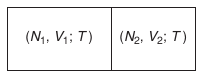
\includegraphics[width=5cm]{images/mixing-2gases.png}
	    \caption{Mezcla de dos gases ideales.}
	    \label{fig:gibbs-paradox}
	  \end{figure}
	  
	\item La consecuencia física del arreglo de Gibbs es que se está 
	reduciendo el número de microestados accesibles por el sistema 
	en un factor $N!$. La justificación de esto es que estamos lidiando
  con partículas idénticas que son indistinguibles, por consiguiente
  no tiene sentido etiquetar individualmente a cada una de las
  partículas. Todo lo que podemos contar es la distribución 
  sobre los estados de energía.
\end{itemize}

\section{Elementos de la teoría de los ensambles}
\begin{itemize}
	\item Un microestado de un sistema clásico, en un tiempo $t$, está
	definido por las posiciones y momenta de todas las partículas
	que constituyen al sistema.
	\item Las coordenadas $(q_i,p_i)$ representan un punto en 
	un espacio de $6N$ dimensiones conocido como el espacio de fases.
	\item Función de densidad $\rho(q,p;t)$: para describir mejor 
	los ensambles de microestados en los que se puede encontrar
	un sistema. Esta función es tal que el número de puntos 
	representativos dentro del elemento de volumen $d^{3N}qd^{3N}p$
	alrededor del punto $(q,p)$ del espacio de fases está dado por 
	el proudcto $\rho(q,p;t)d^{3N}qd^{3N}p$.
	\item El promedio del ensamble $\expval{f}$ de una cantidad
	física $f(q,p)$ está dado por 
	\begin{align}
	\expval{f}=
	\frac{\int f(q,p)\rho(q,p;t)d^{3N}qd^{3N}p}{\int \rho(q,p;t)d^{3N}qd^{3N}p}
	\end{align}
	
	\item \textbf{Teorema de Liouville:} Consideremos una región de
	volumen arbitrario $\omega$, cuya superficie la vamos a denotar
	por $\sigma$, como se ve en la \Fref{fig:liouville}. 
	Entonces, la tasa a la que el número de puntos 
	representativos en este elemento de volumen aumenta con 
	el tiempo es
	\begin{align}
	\pdv{t}\int_{\omega} \rho d\omega.
	\end{align}
	Por otro lado, el flujo hacia afuera de $\omega$ está dado por 
	\begin{align}
	\int _{\sigma}\rho \vb{v}\cdot \vb{\hat{n}}d\sigma.
	\end{align}
	Por el teorema de la divergencia (que no tengo fresco en el momento
	que estoy escribiendo esto \janote{OJO}) tenemos 
	\begin{align}
	\int _\omega \div{\rho \vb{v}}d\omega.
	\end{align}
	En vista que no hay fuentes ni sumideros
	\begin{align}
	\pdv{t}\int_{\omega} \rho d\omega=-\int _\omega \div{\rho \vb{v}}d\omega,
	\end{align}
	por lo que 
	\begin{align}
	\int _{\omega}\qty(\pdv{\rho}{t}+\div{\rho\vb{v}})d\omega=0.
	\end{align}
	Por lo cual, inmediatamente se tiene 
	\begin{align}
	\pdv{\rho}{t}+\div{\rho\vb{v}}=0,
	\end{align}
	y esta ecuación es conocida como la ecuación de continuidad. 
	Trabajando más esta ecuación 
	\begin{align}
	\pdv{\rho}{t}+\sum_{i=1}^{3N}
	\qty(\pdv{\rho}{q_i}\dot{q}_i+\pdv{\rho}{p_i}\dot{p}_i)+
	\rho \sum_{i=1}^{3N}
	\qty(\pdv{\dot{q}_i}{q_i} + \pdv{\dot{p}_i}{p_i})=0.
	\end{align}
	\h{Recordatorio eqs. de Hamilton:} 
	\begin{align}
	\dot{q}_i&=\pdv{H(q_i,p_i)}{p_i}\\
	\dot{p}_i&=-\pdv{H(q_i,p_i)}{q_i}.
	\end{align}
	Usando la ecuaciones de Hamilton notamos que 
	el tercer término en la ecuación de continuidad se hace cero,
	por consiguiente llegamos al resultado 
	conocido como el \h{teorema de Liouville}:
	\begin{align}
	\pdv{\rho}{t}+\{\rho,H\}=0,
	\end{align}
	donde $\{\rho,H\}$ es el bracket de Poisson. La consecuencia 
	física de este teorema es que las trayectorias en el espacio de 
	fases se mueven de la misma manera que un fluido 
	incompresible.
	\begin{figure}
	  \centering
	  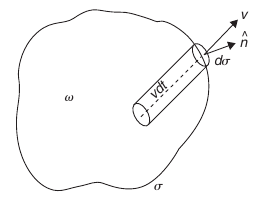
\includegraphics[width=5cm]{images/phase-space.png}
	  \caption{Elemento de volumen en el espacio de fases.}
	  \label{fig:liouville}
	\end{figure}
	
	\item \textbf{Ensamble canónico:} $E=$ cte.
	
	\item \textbf{El ensamble microcanónico:}
	El macroestado del ensamble microcanónico de un sistema está 
	definido por el número de moléculas $N$, el volumen $V$ y la 
	energía $E$. El ensamble microcanónico es una colección de
	sistemas para los cuales la función de densidad $\rho$ está 
	dada por 
	\begin{align}
	\rho(q,p)=\text{cte.}\hspace{1cm}
	\text{si} \hspace{2mm}
	\qty(E-\frac{1}{2}\Delta)\leq
	H(q,p)\leq
	\qty(E+\frac{1}{2}\Delta).
	\end{align}
	
	\item El resultado fundamental es llegar a la \textbf{energía 
	libre de Helmholtz!!!!} (ver sec. 3.3 Pathria)
	
	\item El formalismo del ensamble microcanónico y canónico son equivalentes.
	
	\item \textbf{Teorema de equipartición:} (revisar notas en Drive para la 
	deducción matemática) cada término armónico en el Hamiltoniano 
	transformado de un sistema contribuye $1/2kT$ a la energía 
	interna del sistema. Dicho de otro modo, cada grado de libertad 
	aporta la misma cantidad al valor esperado de la energía del sistema 
	total. \textbf{No obstante}, el teorema de equipartición es válido 
	para valores de temperatura muy altos, osea cuando los 
	grados de libertad relevantes del sistema pueden 
	ser excitados libremente.
	
	\item \textbf{Teorema del virial:} (revisar notas en Driva para la 
	deducción) 
	\begin{align}
	-\expval{\sum_iq_i\dot{p_i}}=3NkT,
	\end{align}
	donde
	\begin{align}
	\mathcal{V}=-3NkT,
	\end{align}
	es	llamado el 'virial' del sistema.
	Cuando se considera a un gas ideal esto se reduce a la relación 
	clásica:
	\begin{align}
	\mathcal{V}=-2K,
	\end{align}
	con $K$ la energía cinética del sistema.	
\end{itemize}

\subsection{Osciladores armónicos}
Asumiendo osciladores armónicos en una dimensión el hamiltoniano
$H$ del sistema es 
\begin{align}
H(q_i,p_i)=\sum_i\frac{1}{2}m\omega^2q_i^2+\frac{1}{2m}p_i^2.
\end{align}
Al calcular la función de partición $\mathcal{Z}$ de un oscilador armónico
\begin{align}
\mathcal{Z}&=\int _{-\infty}^{\infty}\int _{-\infty}^{\infty}
\exp\qty[-\beta\qty(\frac{1}{2}m\omega^2q^2+\frac{1}{2m}p^2)]
\frac{dqdp}{h}\nonumber\\
&=\frac{1}{h}\qty(\frac{2\pi}{\beta m\omega^2})^{1/2}
\qty(\frac{2\pi m}{\beta})^{1/2}=
\frac{1}{\beta\hbar\omega}=\frac{kT}{\hbar\omega}.
\end{align}
De manera que entonces la función de partición del sistema 
completo es 
\begin{align}
\mathcal{Z}=\qty(\frac{kT}{\hbar\omega})^N.
\end{align}
La energía libre de Helmholtz está dada por 
\begin{align}
A&=-kT\ln \mathcal{Z}\nonumber\\
&=-NkT\ln\qty(\frac{kT}{\hbar\omega}).
\end{align}
De manera que las otras variables termodinámicas son
\begin{align}
S&=-\qty(\pdv{A}{T})_{N,V}\nonumber\\
&=Nk\qty[\ln\qty(\frac{kT}{\hbar\omega})+1]
\end{align}
y 
\begin{align}
U&=\pdv{\ln\mathcal{Z}}{\beta}\nonumber\\
&=NkT.
\end{align}


\bibliographystyle{abbrv}
\bibliography{references}
\end{document}


